\chapter{Omega-X}
\section{Pre-planing(part 1)}
\subsection{Ideas \& Overarching Plan}
\par Start with replicating 1D thermal fluid model, then start with more complex models, then experiment with other ways to do it, then dive deeper into the mathematics and hopefully come up with something(maybe metriplectic integrator), then create a code base, compare these systems to other traditional models, and create tokomak simulation(maybe, not sure if possible yet) that is it so far. Hopefully these ideas will evolve. 

Basically, the whole idea is to create a Flash-X like project with Metriplectic formulism underlying the the dynamics rather than lagrangian or Newtonian. Obviously much simpler though.

\subsection{Metriplectic 4-bracket algorithm for constructing thermodynamically consistent
 dynamical systems}
\subsubsection{Math}
1: Identify dynamical variables
2: Propose energy and entropy functionals
3: Find Poisson bracket ${F, G}$ for which entropy $S$ is a Casimir invariant, ${F, S} = 0 \forall F$
4: Construct metriplectic 4-bracket (F, K; G, N) via Kulkarni-Nomizu product by a new method that separates local thermodynamics from phenomenological quantities, giving the EoMs as Poisson bracket + 4-bracket

To find the $\Sigma$ and $M$ a new method is derived. 
$$\partial_t \xi^\alpha= \{\xi^\alpha , H\} + \nabla \cdot J^\alpha$$
$\alpha = 1, 2... N-1$
$$\partial_t \xi^N= \{\xi^N , H\} + \nabla \cdot J^N+Z_\alpha \cdot \tilde{L}^{\alpha \beta} \cdot Z_\beta$$
where $\xi_N = \sigma$, the entropy density. Above splits Hamiltonian and conservative.
Which leads to:
$$M(dF, dG)=F_{\xi N}G_{\xi N}$$
$$\Sigma(dF, dG)=\nabla F_{\xi \alpha }\frac{L^{\alpha \beta}}{H_{\xi N}}\nabla (G_{\xi \beta})$$
\subsection{A thermodynamically consistent discretizations of 1D thermal-fluid
models using their metriplectic 4-bracket structure}
\subsubsection{Math}
Edit: so I don't keep forgetting, $\rho$ is mass density, $m$ is momentum density, and $\sigma$ is entropy density. Then for the thermodynamic quantities: $\eta$ is specific entropy, $u$ is velocity, and $T$ is temperature 
 Let $V_h = v_h \subset H^1(\Omega)$ be the degree-p continuous
 Galerkin finite element space defined over a uniform grid, $\tau_h $, on Ω: i.e.
 $$V_h = {v_h  \in H^1(\Omega) : v_h|K \in P_p(K), \forall K \in T_h}$$
  The discretizations is accomplished
 using the method of lines by positing that all dynamical fields have spatial dependence modeled
 in this Galerkin subspace. However, rather than discretizing the equations of motion themselves,
 we discretize the weak forms implied by the metriplectic formulation.
\\
 Let $(\rho_h. m_h. \sigma_h) \in V_h \times V_h \times V_h$
 So that the discretized Hamiltonian and entropy can be given as:
 $$H^h[\rho_h. m_h. \sigma_h]= \int_\Omega [\frac{1m^2_h}{2 \rho_h}+\rho_h U (\rho_h, \frac{\sigma_h}{\rho_h}]dx$$
 $$S^h[\sigma_h]=\int_\Omega \sigma_h dx$$
 Then the Metriplectic 4 Bracket can be expressed through:
 $$(F^h, K^h, G^h, N^h)_h = -\frac{1}{\text{Re}} \int_{\Omega} \frac{1}{T_h} \left[ \left( K^h \partial_x F^h_{m_h} - F^h \partial_x K^h_{m_h} \right) \right], $$
 $$\left( N^h \partial_x G^h_{m_h} - G^h \partial_x N^h_{m_h} \right)  \\
 +, $$
$$ \frac{1}{\text{Pr} \gamma - 1} \frac{1}{T_h} \left( K^h \partial_x F^h - F^h \partial_x K^h \right) \left[ \left( N^h \partial_x G^h - G^h \partial_x N^h \right) \right] \, dx $$
\\
Then the poission bracket is thus:
\begin{align*}
\{F^h, H^h\}_h(u_h)= - (m_h \partial_x u_h, \phi_m)_{L^2} + (m_h u_h, \partial_x , \phi_m)_{L^2} - \\ (\rho_h \partial_x \eta_h, \phi_m)_{L^2}  + (\rho_h u_h, \partial_x , \phi_\rho)_{L^2} - (\sigma_h\partial_x T_h, \phi_m)_{L^2} + (\sigma_h u_h, \partial_x, \phi_\sigma)_{L^2}
\end{align*}
Now, one thing I will say is that this is not technically a Poisson bracket, because it is fails to satisfy the Jacobi identity. This is because it is impossible(or at least nobody has figured out a way to discretize fluid poission brackets.

To then find equations of motion, adding them together $F^h=\{F^h, H^h\}_h+(F^h, H^h; S^h, H^h)_h$ where $F^h$ is the observable. 

In the case of momentum we must let $\phi_\rho = \phi_\sigma = 0$ so that only $\phi_\rho$ the momentum test function in the finite element(FE) test space $V_h$.

\begin{align*}
    (\phi_m, \partial_tm_h) + (m_h\partial_xu_h, \phi_m)_{L^2} - (m_h u_h, \partial_x, \phi_m)_{L^2}
    + (\rho_h \partial_x \eta_h, \phi_m)_{L^2} + (\sigma_h\partial_xT_h \phi_m)_{L^2} +
    \frac{1}{Re}(\partial_xu_h, \partial_x, \phi_m)_{L^2} = 0 
\end{align*}
\\
Next, I will have $\phi_m=\phi_\sigma=0$ to get continuity equations:
\\
\begin{align*}
    (\phi_\rho, \partial_g \rho_h)_{L^2}-(\rho_hu_h, \partial_x \phi_\rho)_{L^2}
\end{align*}

Finally the entropy equation is derived in a similar fashion:

\begin{align*}
    (\phi_\sigma, \partial_g \sigma_h)_{L^2}-(\sigma_h u_h, \partial_x \phi_\sigma)_{L^2}+\frac{1}{Re}[(\frac{(\partial_x u_h)^2}{T_h}, \phi_\sigma)_{L^2}-\frac{1}{Pr}\frac{\gamma}{\gamma-1}[(\frac{\partial_x T_h}{T_h}, \partial_x\phi_\sigma)_{L^2}-(\frac{(\partial_x T_h)^2}{T_h^2}, \phi_\sigma)_{L^2} ]]
\end{align*}

To prove energy conservation
$$(\frac{u^{n+1}_h-u^n_h}{\Delta t}, \delta h_h)=\frac{H(u^{n+1}_h)-H(U^n_h)}{\Delta t} = 0$$
Positive entropy production can be found through:
$$\frac{s^{n+1}_h-s^n_h}{\Delta t} = \frac{1}{Re}[(\frac{(\partial_x u^n_h)^2}{T^n_h},1)_{L^2}+\frac{1}{Pr}\frac{\gamma}{\gamma-1}\frac{(\partial_x T^n_h)^2}{T^n_h},1)_{L^2}]\geq 0$$


Let's figure out all we need to find for each equation, starting with momentum. 
Start with $M_{ii}=\phi_m$, this should be equal to dx, but I will confirm. Also need the time derivative of the momentum variational, $u_h$ variational, $\rho_h$ variational, $T_h$, $\eta_h$, and $\frac{1}{Re}$, reynolds number, decide later

$$M_{ii}=dx$$
$$u_h=(\rho_h, m_h, \sigma_h)$$
$\rho_h$, $T_h$, and $\eta_h$ are the respective fields, initialized simply and evolved through the equation.
Obviously $\rho_h, m_h,$ and $\sigma_h$ evolve through their metriplectic equations of "motion."
$T_h$, $\eta_h$, are evolved through these equations:
$$(\eta_h + \frac{m^2_h}{2\rho^2_h}-U(\rho_h, \frac{\sigma_h}{\rho_h})-\rho_h \partial_1 U(\\rho_h, \frac{\sigma_h}{\rho_h})+\frac{\rho_h}{\sigma_h}\partial_2U(\rho_h, \frac{\sigma_h}{\rho_h}, \phi_\eta)_{L^2}=0$$
$$(u_h-\frac{m_h}{\rho_h},\phi_u)=0$$
$$(T_h-\partial_2U(\rho_h, \frac{\sigma_h}{\rho_h})\phi_T)_{L^2}=0$$
\\
Nothing new is added in continuity
\\
Entropy adds: $Pr$ and $\gamma$
\subsubsection{Coding}
The first thing is to use a Galerkin Method for projecting PDEs into a finite-dimensional function space. (can base off of Firedrake, FEniCS, Galerkin, or another) $M_{ii}$ in mesh.f90

The second thing to do is to initialize the parameters and states(use mesh to calculate field) in states.f90
($Pr$, $Re$, $\gamma$ for constants; initialize ($\rho_h, \sigma_h, m_h, \eta_h, T_h, u_h$)


Then functionals: calculates pointwise functional derivatives of the Total Hamiltonian and Entropy. in functionals.f90
(Update $\rho_h, \sigma_h, m_h, u_h$)

EOS.f90 is used to update the thermodynamic points($\eta_h, T_h$)

Time step the program, by using Gauss-Legendre implicit Runge-Kutta methods in time\_integration.f90

Run the Program(using the driver and makefile)

Input the outputs in io.f90

Some notes: $(f,g)_{L^2}=\int_\Omega f(x) \cdot g(x)$

An example would be, for a point in the momentum equation $(\phi_m, \partial_t m_h)_{L^2}$, or the mass matrix times the derivative of momentum functional as a function of time. Thus it makes it so $\phi_m=M_{ii}=dx$ thus, $(\phi_m, \partial_t m_h)_{L^2}=dx\cdot\frac{m_h}{\partial t}$

\subsubsection{Future Work}
The paper presents several ways to improve, or at least look into improving through future work.

Mainly, they mention that many different structure preserving methods exist and may be more suitable.

I also need to figure out how to make this codebase work for more examples



\subsection{Metriplectic Framework for
 Dissipative Magneto-Hydrodynamics}
\subsubsection{My Introduction}
In my time trying to figure out how to numerically solve metriplectic equations, someone beat me to dissipative magneto-hydrodynamics. Oh well, I can build off of.

Beyond that, the abstract introduces the paper better than I could,
" The metriplectic framework, which permits to formulate an algebraic structure for dissipative
 systems, is applied to visco-resistive Magneto-Hydrodynamics (MHD), adapting what had already
 been done for non-ideal Hydrodynamics (HD). The result is obtained by extending the HD sym
metric bracket and free energy to include magnetic field dynamics and resistive dissipation. The correct equations of motion are obtained once one of the Casimirs of the Poisson bracket for ideal MHD is identified with the total thermodynamical entropy of the plasma. The metriplectic frame work of MHD is shown to be invariant under the Galileo Group. The metriplectic structure also permits to obtain the asymptotic equilibria toward which the dynamics of the system evolves. This scheme is finally adapted to the two-dimensional incompressible resistive MHD, that is of major use in many applications."
\subsubsection{Notes on introduction}
They have an interesting word choice, "with its noble descendants of path integral representations," or Algebrization of dynamical systems appears to be the final destination of that virtuous route.

MSTDOF means "microscopic, statistically treated, degrees of freedom"

In this introduction they derive the metriplectic existence quite simply.
Starting with the poission bracket 
$$\dot{f}=\{f,g\}$$
In this case
$$0= \{S,H\}$$
Thus it is the Casimir functionals of the Poisson bracket
$$\{C,f\}=0 \forall f$$
From here we can define the Hamiltonian free energy. 
$$F=H+\lambda C $$
Where $\lambda$ is an arbitrary constant left. In MSTDOF, it is the minus of the tempeture.

To then expand the system, $\langle\langle f,g \rangle \rangle$ via $F$. So that $\langle\langle f, g\rangle \rangle=\{f,h\} + (f,g)$ and $(f,g)$ is symmetric, bilinear and semi-definite.

Evolution is then given by
$$\dot{f}=\langle\langle f, F\rangle \rangle$$
(the symmetric bracket $(f,g)$ will be defined so to cancel out the presence of the coefficient
 $\lambda$, removing it from the equations of motion).

 $(f,g)$ is defined so that $H$ is conserved.
 $$(H, f) = 0 \forall f$$
 Thus metriplectic evolution reads:
 $$\dot{f}=\{f,H\}+\lambda(f,C)$$
 The Casimir to mimic entropy undergoes an evolution described by:
 $$\dot{C}=\lambda(C,C)$$
 \\
 Now, I like this introduction. Clearly showing the basic understanding on Metriplectic dynamics.
 \subsection{METRIPLECTIC FORMULATION OF VISCO-RESISTIVE MHD}
 The system observed is fully ionized plasma. Where dissipation takes place due to the finite viscosity and resistivity of the fluid. Also, heat conductivity is finite. Here is the SO(3)-covariant form.(expressing physical equations in a way that is invariant under rotations in three-dimensional space)
 \begin{align*}
\partial_t \rho + \partial_i (\rho u^i) &= 0 \\
\partial_t B^i + \varepsilon^{ijk} \partial_j E_k &= 0, \quad \partial_i B^i = 0 \\
\partial_t (\rho u^i) + \partial_j (\rho u^i u^j + p \delta^{ij}) &= \varepsilon^{ijk} J_j B_k + \partial_j (\eta \, \partial_j u^i) \\
\partial_t s + \partial_i (s u^i) &= \frac{\eta}{T} \partial_i u^j \partial_i u^j + \frac{\kappa}{T^2} \partial_i T \partial_i T + \frac{\mu}{T} J^i J^i
\end{align*}
There is quite a bit to this equation, but I will move on.

One thing I will add is a new notation. $\dot{H}\overset{\partial}{=}0$, it simply means that means that $\dot{H}$ and 0 only differ by a boundary term.

They then describe the poission bracket for ideal MHD(when dissipation does not happen, thus traditional poission bracket).

This equation has multiple Casimir observables. The paper mentions:
$$C[\rho, s]=\int_\mathbb{D}\rho\varphi(s)d^3x$$
Which within is both the total mass and entropy.
$$M[\rho]=\int_\mathbb{D}\rho d^3x$$
$$S[\rho,s]=\int_\mathbb{D}\rho s d^3x$$
Thus, mass and entropy are conserved. There are some other, but obviously for this purpose, use the entropy.

Taking the dissipative equations from the to combine $D=(\vec{D}^\rho, \vec{D}^v, \vec{D}^B, \vec{D}^s)$ something called an 8-uple. So we must want to define our metriplectic bracket as $\psi = (\psi, D)$ where $\psi$ is the dynamic variables.

Uhm.. I just realized this wasn't the paper I thought it was. Good read, but I don't think I will continue these notes.
\subsection{A least Action principle for visco-resistive Hall Magnetohydrodynamic with metriplectic reformulation}
\subsubsection{Abstract}
The abstract persented says,

"We present a new variational formulation for Viscous and resistive Hall Magnetohydrodynamic. We first find a variational principle for ideal HMHD by applying the physical assumptions leading to HMHD at the lagrangian level, and then we add the viscous and resistive terms by the means of constrained variations. We also provide a metriplectic reformulation of our formulation, based on two canonical Lie-Poisson brackets for the ideal part and metric 4-brackets for the dissipative part."

They then go into all of these, I will begin with the Metriplectic for notes alone.
\subsubsection{Metriplectic bracket, Hamiltonian and Entropy for Viscoresistive Hall MHD}
They use the Inclusive curvaturelike tensor found in Morrison's recent work. Where the dissipation is included using a 4-bracket that have the same symmetries as a curvature tensor.

They take the assumption that the viscous  tensor can be found to be 
$$\sigma=\Lambda \nabla u_i$$
Where $\Lambda$ is symmetrize and positive.
\subsection{Variational discretizations of viscous and resistive
 magnetohydrodynamics using structure-preserving finite
 elements}
 \subsubsection{Abstract}
 We propose a novel structure preserving discretization for viscous and resistive magnetohy
drodynamics. We follow the recent line of work on discrete least action principle for fluid and
 plasma equation, incorporating the recent advances to model dissipative phenomena through
 a generalized Lagrange-d’Alembert constrained variational principle. We prove that our semi
discrete scheme is equivalent to a metriplectic system and use this property to propose a Poisson
 spliting time integration. The resulting approximation preserves mass, energy and the diver
gence constraint of the magnetic field. We then show some numerical results obtained with our
 approach. We first test our scheme on simple academic test to compare the results with estab
lished methodologies, and then focus specifically on the simulation of plasma instabilities, with
 some tests on non Cartesian geometries to validate our discretization in the scope of tokamak
 instabilities.

 
 This paper
\section{part 2}
\subsection{Coding(1D fluid)}
\paragraph{Introduction}
My first step to creating my codebase is to create it for the simplest form. This is specifically made for the purpose of figuring things out, documenting it, and such things. So, I will be writing down each file.

\paragraph{mesh\_1d}
Obviously, this mesh program creates the mesh for the program. The size $N$, the nodes $x\_nodes$ and the mass matrix $M_{ii}$. The rest are self explanatory but I will go into what the mass matrix is. It represents the discrete inner product of basis functions.
$$M_{ii}=(\phi_i,\phi_j)_{L^2}=\int_\Omega \phi_i(x)\phi_j(x)dx$$
So, $M_{ii} $ becomes a metric tensor for program. It turns continuous inner products into discrete sums over coefficients.

It can be approximated through the "lumped mass matrix" where $M_{ii}=dx$
Though, I use the trapezoidal mass matrix:
$$M_{ii}(1) = 0.5d0 * dx $$
$$ M_{ii}(N) = 0.5d0 * dx$$
$$M_{ii}(2:N-1) = dx$$
For more information visit, \url{https://arxiv.org/pdf/2008.03883}
\begin{lstlisting}[style=FORTRAN, caption=mesh\_1d.f90]
module mesh_1d
  implicit none
  private
  public :: initialize_mesh, x_nodes, dx, N, Mii

  ! Parameters
  integer, parameter :: N = 100         ! Number of spatial grid points (nodes)
  real(8), parameter :: L = 1.0d0       ! Length of the domain

  ! Mesh data
  real(8), dimension(N) :: x_nodes      ! Coordinates of each mesh node
  real(8) :: dx                         ! Uniform cell spacing

  ! Mass matrix (diagonal approximation here, for full FEM use full M)
  real(8), dimension(N) :: Mii          ! Lumped mass matrix diagonal

contains

  subroutine initialize_mesh()
    integer :: i

    dx = L / (N - 1)

    ! Initialize node positions
    do i = 1, N
      x_nodes(i) = (i - 1) * dx
    end do

    ! Lumped mass matrix: each diagonal entry is dx
    Mii = dx

    ! Uncomment below to use trapezoidal mass matrix
    Mii(1) = 0.5d0 * dx
    Mii(N) = 0.5d0 * dx
    Mii(2:N-1) = dx

  end subroutine initialize_mesh


end module mesh_1d 
\end{lstlisting}

\paragraph{states\_1d}
States then initializes the constants and fields.
First the constants(parameters) used throughout the code. Re, Reynolds numbers. $\gamma$, compression of the fluid. $Pr$, Prandtl number, ratio of viscous to thermal diffusion.

Then, it initializes the discretion fields of entropy, momentum, mass, temperature, and specific entropy.

This should be modularized for the future to make this codebase iterative.

Now, what exactly to do. I think for this, have constants in a separate one. Then for the fields, I am not sure at this moment.
\begin{lstlisting}[style=FORTRAN, caption=states\_1d.f90]
module states_1d
  use mesh_1d
  implicit none
  private
  public :: m_h, rho_h, sigma_h, eta_h, T_h
  public :: initialize_states

  ! Field arrays
  real(8), allocatable :: m_h(:)       ! Momentum density
  real(8), allocatable :: rho_h(:)     ! Mass density
  real(8), allocatable :: sigma_h(:)   ! Entropy density
  real(8), allocatable :: eta_h(:)     ! Specific entropy (diagnostic)
  real(8), allocatable :: T_h(:)       ! Temperature (diagnostic)
  real(8), parameter, public :: gamma = 1.4
  real(8), parameter, public :: Pr = 0.71
  real(8), parameter, public :: Re = 1000.0

contains

  subroutine initialize_states()
    implicit none
    integer :: i

    ! Allocate fields
    allocate(m_h(N))
    allocate(rho_h(N))
    allocate(sigma_h(N))
    allocate(eta_h(N))
    allocate(T_h(N))

    ! Set initial conditions (example: Gaussian density bump)
    do i = 1, N
      rho_h(i) = 1.0d0 + 0.2d0 * exp(-100.0d0 * (x_nodes(i) - 0.5d0)**2)
      eta_h(i) = 1.0d0
      sigma_h(i) = rho_h(i) * eta_h(i)
      m_h(i) = 0.5d0
      T_h(i) = (0.4d0) * eta_h(i)  ! Ideal gas ! Uses EOS
    end do

  end subroutine initialize_states

end module states_1d
\end{lstlisting}
\paragraph{projection\_matrix\_1d}
Here the creation of two subroutines to simplify future calculations.
First, initialize\_projection\_matrix(), that simply creates matrix.
Next, apply\_weak\_derivative(f, d\_proj). This does:
$$proj=\sum_{i=1}^n(\sum_{j=1}^nD_{i,j})*f$$
Where $f$ is the observable.
For future work, I think all I need to do for this one is create multiple for different dimensions.
\begin{lstlisting}[style=FORTRAN, caption=projection\_matrix\_1d.f90]
module projection_matrix_1d
  use mesh_1d
  implicit none
  real(8), allocatable :: D(:,:)
  public :: initialize_projection_matrix, apply_weak_derivative

contains

  subroutine initialize_projection_matrix()
    integer :: i
    real(8) :: dphi_dx
    if (allocated(D)) then
      deallocate(D)
    end if

    allocate(D(N, N))
    D = 0.0d0

    dphi_dx = 1.0d0 / dx

    ! Loop over elements and assemble D
    do i = 2, N-1
      ! Local contributions from basis functions over each element
      D(i, i-1) = -dphi_dx / 2.0d0
      D(i, i  ) =  0.0d0
      D(i, i+1) =  dphi_dx / 2.0d0
    end do

    ! Optional: Neumann (zero derivative) at boundaries
    D(1,:) = 0.0d0
    D(N,:) = 0.0d0
  end subroutine initialize_projection_matrix

  ! Applies D to f to compute (phi_i, partial_x f)
  subroutine apply_weak_derivative(f, d_proj)
    implicit none
    real(8), intent(in)  :: f(N)
    real(8), intent(out) :: d_proj(N)
    integer :: i

    d_proj = 0.0d0
    do i = 1, N
      d_proj(i) = sum(D(i,:) * f(:))
    end do
  end subroutine apply_weak_derivative

end module projection_matrix_1d
\end{lstlisting}
\paragraph{mass\_1d}

\begin{lstlisting}[style=FORTRAN, caption=mass\_1d.f90]
module mass_1d
  use mesh_1d
  use projection_matrix_1d
  implicit none
contains

  subroutine compute_mass_flux(N, rho_h, u_h, rho_rhs)
    integer, intent(in) :: N
    real(8), intent(in) :: rho_h(N), u_h(N)
    real(8), intent(out) :: rho_rhs(N)
    real(8) :: flux(N)
    integer :: i

    ! Compute flux
    do i = 1, N
      flux(i) = rho_h(i) * u_h(i)
    end do

    ! Apply weak derivative
    call initialize_projection_matrix()
    call apply_weak_derivative(flux, rho_rhs)

    ! Divide by dx
    do i = 1, N
      rho_rhs(i) = -rho_rhs(i) / dx
    end do

    ! Boundary conditions
    rho_rhs(1) = 0.0d0
    rho_rhs(N) = 0.0d0

  end subroutine compute_mass_flux

end module mass_1d
\end{lstlisting}
\paragraph{momentum\_1d}
\begin{lstlisting}[style=FORTRAN, caption=momentum\_1d.f90]
module momentum_1d
  use states_1d, only: Re
  use mesh_1d
  use projection_matrix_1d
  implicit none
contains

  subroutine compute_momentum_rhs(N, rho_h, m_h, sigma_h, eta_h, T_h, rhs_m)
    integer, intent(in) :: N
    real(8), intent(in) :: rho_h(N), m_h(N), sigma_h(N), eta_h(N), T_h(N)
    real(8), intent(out) :: rhs_m(N)
    real(8) :: u_h(N), du_proj(N), mu(N), dmu_proj(N), deta_proj(N), dT_proj(N)
    integer :: i

    ! Compute velocity
    do i = 1, N
      if (rho_h(i) > 1.0d-12) then
        u_h(i) = m_h(i) / rho_h(i)
      else
        u_h(i) = 0.0d0
      end if
    end do

    ! Apply weak derivatives
    call initialize_projection_matrix()
    call apply_weak_derivative(u_h, du_proj)
    do i = 2, N-1
      mu(i) = m_h(i) * u_h(i)
    end do
    call apply_weak_derivative(mu, dmu_proj)
    call apply_weak_derivative(eta_h, deta_proj)
    call apply_weak_derivative(T_h, dT_proj)

    ! Compute RHS
    do i = 2, N-1
      rhs_m(i) = 0.0d0
      rhs_m(i) = rhs_m(i) - m_h(i) * du_proj(i) * dx
      rhs_m(i) = rhs_m(i) + dmu_proj(i) * dx
      rhs_m(i) = rhs_m(i) - rho_h(i) * deta_proj(i) * dx
      rhs_m(i) = rhs_m(i) - sigma_h(i) * dT_proj(i) * dx
      rhs_m(i) = rhs_m(i) - (1.0d0 / Re) * du_proj(i) * dx
    end do

    ! Boundary conditions
    rhs_m(1) = 0.0d0
    rhs_m(N) = 0.0d0

  end subroutine compute_momentum_rhs

end module momentum_1d
\end{lstlisting}
\paragraph{entropy\_1d}
\begin{lstlisting}[style=FORTRAN, caption=entropy\_1d.f90]
module entropy_1d
  use states_1d
  use mesh_1d
  use projection_matrix_1d
  implicit none
contains

  subroutine compute_entropy_rhs(N, sigma_h, u_h, T_h, rhs_sigma)
    implicit none
    ! Dummy arguments
    integer, intent(in) :: N
    real(8), intent(in) :: sigma_h(N), u_h(N), T_h(N)
    real(8), intent(out) :: rhs_sigma(N)

    ! Local variables
    real(8) :: flux(N), dx_u(N), dx_T(N)
    real(8) :: visc_prod(N), heat_prod(N), heat_grad(N), heat_term(N)
    integer :: i

    ! Compute flux
    do i = 1, N
      flux(i) = sigma_h(i) * u_h(i)
    end do

    ! Apply weak derivatives
    call initialize_projection_matrix()
    call apply_weak_derivative(flux, rhs_sigma)
    call apply_weak_derivative(u_h, dx_u)
    call apply_weak_derivative(T_h, dx_T)

    ! Viscous and thermal terms
    do i = 1, N
      visc_prod(i) = (dx_u(i)**2) / T_h(i)
      heat_grad(i) = dx_T(i) / T_h(i)
      heat_prod(i) = (dx_T(i)**2) / (T_h(i)**2)
      heat_term(i) = (gamma / (gamma - 1.0d0)) * (heat_prod(i) - heat_grad(i) / dx)
      rhs_sigma(i) = rhs_sigma(i) - (1.0d0 / Re) * visc_prod(i) * dx
      rhs_sigma(i) = rhs_sigma(i) - (1.0d0 / (Re * Pr)) * heat_term(i) * dx
    end do

    ! Divide by dx
    do i = 1, N
      rhs_sigma(i) = -rhs_sigma(i) / dx
    end do

    ! Boundary conditions
    rhs_sigma(1) = 0.0d0
    rhs_sigma(N) = 0.0d0

  end subroutine compute_entropy_rhs

end module entropy_1d
\end{lstlisting}
\paragraph{velocity\_1d}
\begin{lstlisting}[style=FORTRAN, caption=velocity\_1d.f90]
module velocity_1d
  use states_1d
  use projection_matrix_1d
  implicit none
contains

  subroutine compute_velocity(N, rho_h, m_h, u_h)
    implicit none

    ! Dummy arguments
    integer, intent(in) :: N
    real(8), intent(in) :: rho_h(N), m_h(N)
    real(8), intent(out) :: u_h(N)

    ! Local variables
    integer :: i
    real(8), parameter :: eps = 1.0d-12  ! Small number to avoid division by zero

    ! Compute velocity safely
    do i = 1, N
      if (rho_h(i) > eps) then
        u_h(i) = m_h(i) / rho_h(i)
      else
        u_h(i) = 0.0d0
      end if
    end do

  end subroutine compute_velocity

end module velocity_1d
\end{lstlisting}

\paragraph{EOS\_1d\_thermal}

\begin{lstlisting}[style=FORTRAN, caption=EOS\_1d\_thermal.f90]
module eos_1d
  use states_1d
  implicit none
  private
  public :: compute_temperature, compute_eta



contains

  !------------------------------------------------------------
  ! Compute temperature T from specific entropy eta
  ! T = (gamma - 1) * eta
  !------------------------------------------------------------
  function compute_temperature(eta_h) result(T_h)
    real(8), intent(in) :: eta_h
    real(8) :: T_h

    T_h = (gamma - 1.0d0) * eta_h
  end function compute_temperature

  !------------------------------------------------------------
  ! Compute specific entropy eta from temperature
  ! eta = T / (gamma - 1)
  !------------------------------------------------------------
  function compute_eta(T_h) result(eta_h)
    real(8), intent(in) :: T_h
    real(8) :: eta_h

    eta_h = T_h / (gamma - 1.0d0)
  end function compute_eta

end module eos_1d
\end{lstlisting}
\paragraph{time\_integrator\_1d}
\begin{lstlisting}[style=FORTRAN, caption=time\_integrator\_1d.f90]
module time_integrator_1d
  use mesh_1d
  use states_1d
  use velocity_1d
  use eos_1d
  use mass_1d
  use momentum_1d
  use entropy_1d
  implicit none
  private
  public :: advance_one_step

contains

  subroutine advance_one_step(dt, u_h, rhs_m, rho_rhs, rhs_sigma)
    real(8), intent(in) :: dt
    real(8), intent(INOUT) :: u_h(N), rhs_m(N), rho_rhs(N), rhs_sigma(N)
    integer :: i

    ! Step 1: Compute velocity
    call compute_velocity(N, rho_h, m_h, u_h)
    
    ! Step 2: calculate tempeture
    do i = 1, N-1
      T_h(i) = compute_temperature(eta_h(i)) 
    end do
    ! step three: calculate Eta
    do i = 1, N-1
      eta_h(i) =compute_eta(T_h(i))
    end do
    ! Step 4: Compute Galerkin RHS terms
    call compute_momentum_rhs(N, rho_h, m_h, sigma_h, eta_h, T_h, rhs_m)
    call compute_mass_flux(N, rho_h, u_h, rho_rhs)
    call compute_entropy_rhs(N, sigma_h, u_h, T_h, rhs_sigma)

    ! Step 5: Advance in time (Euler / RK1)
    do i = 1, N
      m_h(i)     = m_h(i)     + dt * rhs_m(i)
      rho_h(i)   = rho_h(i)   + dt * rho_rhs(i)
      sigma_h(i) = sigma_h(i) + dt * rhs_sigma(i)
    end do

  end subroutine advance_one_step

end module time_integrator_1d
\end{lstlisting}
\paragraph{io\_1d}
\begin{lstlisting}[style=FORTRAN, caption=io\_1d.f90]
module io_1d
  use mesh_1d
  use states_1d
  use velocity_1d
  use time_integrator_1d
  implicit none
  private
  public :: write_state_to_csv

contains

  subroutine write_state_to_csv(filename)
    implicit none
    character(len=*), intent(in) :: filename
    integer :: i
    logical :: wait
    real(8) :: u_h(N)
    integer :: ierr
    
    ! Ensure the output directory exists
    wait = .true.  ! Command should run synchronously
    call execute_command_line("mkdir -p output", wait, ierr)
    if (ierr /= 0) then
        print *, "Error: Could not create output directory!"
        stop
    end if

    ! Compute velocity u = m / rho
    call compute_velocity(N, rho_h, m_h, u_h)

    ! Open file for writing
    open(unit=10, file=filename, status="replace", action="write", form="formatted")

    ! Header
    write(10, '(A)') 'x,rho,m,sigma,u,T,eta'

    ! Data
    do i = 1, N
      write(10, '(F12.6,1x,F12.6,1x,F12.6,1x,F12.6,1x,F12.6,1x,F12.6,1x,F12.6)') &
        x_nodes(i), rho_h(i), m_h(i), sigma_h(i), u_h(i), T_h(i), eta_h(i)
    end do

    close(10)
  end subroutine write_state_to_csv

end module io_1d
\end{lstlisting}
\paragraph{1D\_Thermal\_driver}
\begin{lstlisting}[style=FORTRAN, caption=momentum\_1d.f90]
program omega_x_driver_1d
  use mesh_1d
  use states_1d
  use time_integrator_1d
  use io_1d
  implicit none
  real(8) :: dt, t, t_end
  integer :: step = 1
  real(8), dimension(N) :: u_h, rhs_m, rho_rhs, rhs_sigma
  character(len=100) :: fname
  
  dt = 1.0d-3
  t_end = 1.0d0
  t = 0.0d0
  
  call initialize_mesh()
  call initialize_states()
  u_h = 0.0d0
  rhs_m = 0.0d0
  rho_rhs = 0.0d0
  rhs_sigma = 0.0d0  ! Explicitly initialize rhs_sigma here

  do while (t < t_end)
    call advance_one_step(dt, u_h, rhs_m, rho_rhs, rhs_sigma)
    t = t + dt
    print *, 't = ', t

    if (mod(step, 100) == 0) then
        write(fname, '(A,I4.4,A)') "output/state_", step, ".csv"
        call write_state_to_csv(fname)
    end if

    step = step + 1
  end do
end program omega_x_driver_1d
\end{lstlisting}
\subsubsection{Plans}
I have now create it in its most basic form, here are my next steps.

Break states up into constants and fields(multi-dimensional fields)

Make operators folder for projection, weak derivative, boundary conditions

Add checks(mainly energy conservation)

Upgrade time integration,(figure out)

Make different spacial discretization

More boundary conditions

Add more physics

Though, the main thing I need to work on is module registry + driver pattern. 
\section{part 3}
\subsection{Notes}
\subsubsection{Notes on module FORTRAN}
I should have a main driver like:
\begin{lstlisting}[style=FORTRAN, caption=Omegax.f90]
program Omegax
	use Driver_module
	implicit none

	call Driver_init()
	call Driver_evolve()
	call Driver_finalize()

end program Omegaz
\end{lstlisting}

There should also be a a config file, saying which modules should be used, and a python script capable of parsing this registery file.
Config would also be where parameters would be stored.
\subsubsection{Diminsionaless programing}
In the config file I can have a section to input the diminsions.

Then have all variable allocatable based upon the diminsions

then have an allocation based upon such diminsions(either preprocessor or generic shape handling)

Instead of hardcoding loops, create cases for different diminsions.


Generaliz derivatives and fluxes.

Also, while physics sections should be generalized, initializing between 3D, would be beneficial.
\subsubsection{Generalize}
Due to Metriplectics dyanmics complex mathematics, a fully generalized system, like FLASH-X, is impossible. This is because it is a dynamical theory based upon Hamiltonian Mechanics, rather than forces in Newtonian.

I am thinking the way to fix this is to create a symbolic python code to be able to generate the function I need.

Also, since these would be in py
\subsection{Plan}

I think the steps I am going to take are:

1: Develop a python code that can generate the math I need, I would also like for it to be able to read a LaTeX code for it.

2: I need to look into how to create a Config file for my problem at hand

3: Fix integration for this new system

4: 
\subsection{New Structure}
Here is the basic idea of what it should look like and do:
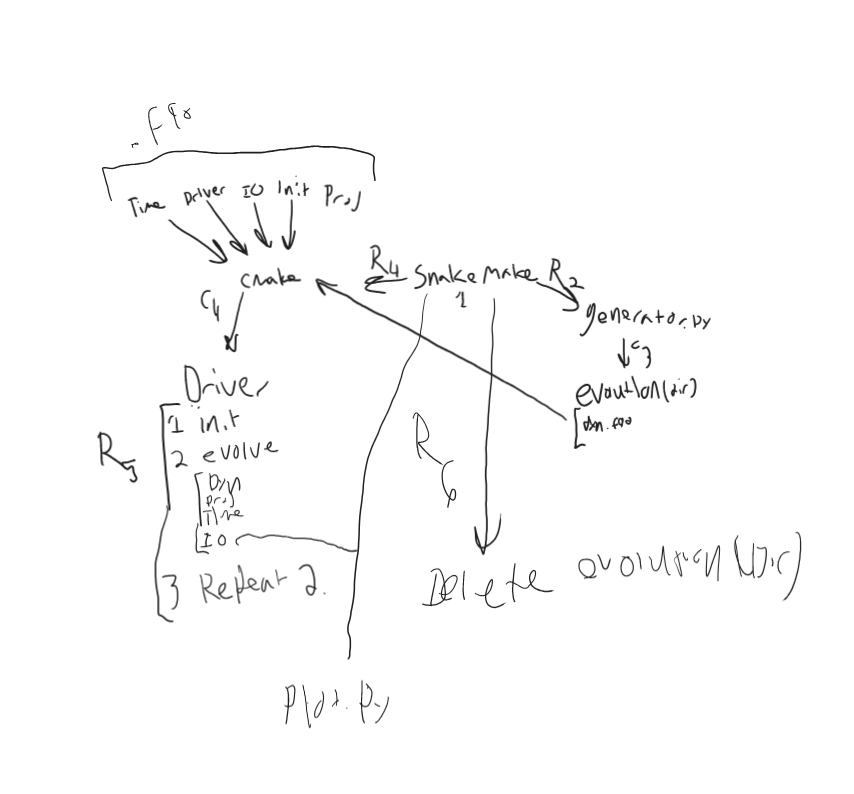
\includegraphics[width=1\textwidth]{../text/part_3/omega-x_overview.png}

